% SKRIV GERNE KOMMENTARER UD FRA "USEPACKAGE" SÅ VI VED HVAD DE GØR :-)
\documentclass[a4paper]{article} 

\usepackage[utf8]{inputenc} % hedder den ikke utf8x? 
\usepackage[danish]{babel}

\usepackage[T1]{fontenc}

\usepackage{csquotes}
\usepackage{verbatim}

\usepackage[margin=2.5cm]{geometry}

\usepackage{hyperref}
\usepackage{soul} % strikeout a line (eg. \st{Hellow world})


\usepackage{graphicx} % Images
\graphicspath{ {./images/} }

\usepackage{listings}
\usepackage[table,xcdraw]{xcolor}
\usepackage{color}

\definecolor{bluekeywords}{rgb}{0.13,0.13,1}
\definecolor{greencomments}{rgb}{0,0.5,0}
\definecolor{turqusnumbers}{rgb}{0.17,0.57,0.69}
\definecolor{redstrings}{rgb}{0.5,0,0}

\usepackage{amsmath}

\title{Diskret Matematik og Algoritmer
\\Ugeopgave 3}
\author{Mads Pontoppidan Haderup (xjr983), Ken Kjøller Andersen (zcj256)\\
og Christian Handest (lzp959)}

\begin{document}
\maketitle % Insert title etc.

%%%%%%%%%%%%%%%%%%%%%%%%%%%%%%%% DEL 1 %%%%%%%%%%%%%%%%%%%%%%%%%%%%%%%%


\pagebreak
\section{DEL 1}

%
%%%% OPGAVETEKST 
%
{\bfseries Afgør for hver af følgende 4 underopgaver, om den ene 
funktion er af lavere størrelsesorden end den anden, eller om de 
to funktioner er af samme størrelsesorden. Argumenter for 
konklusionerne ud fra notesættets regler O1–O9 eller S1–S9.} \\ \\ \\
%
\subsection{DEL 1A}
%
\[ f(n) = \log_{2}(n) \ og \ g(n) = n^2 + 2n \] \\
%
%
%
Det undersøges, om S3 kan benyttes for at finde størrelsesordenen for $f(n)$ og $g(n)$.
\begin{quotation}
S3: "$log_a(x)$ er af lavere størrelsesorden end $x^b$ (a > 1, b > 0)" \\
\end{quotation}
For at benytte S3 skal $f(n)$ og $g(n)$ opfylde betingelserne for at $a > 1$ og $b > 0$. \\
Disse betingelser er opfyldte, da $a = 2$ og $b = 2$. \\ \\
%
Derudover skal det undersøges, om $g(n) = n^2 +2n$ kan skrives på formen $g(n) = n^2$. \\
Da det allerede antages, at $log_2(n)$ < $n^2$, vil $n^2+2n$ kun forøge afstanden
mellem $g(n)$ og $f(n)$. Netop derfor kan vi benytte S1 som siger:

\begin{quotation} \centering S1: "Hvis f(x) er af lavere størrelsesorden end g(x), og g(x) er af lavere størrelsesorden end h(x), så er f(x) af lavere størrelsesorden end h(x)."
\end{quotation}
I vores tilfælde har vi så at $f(n) = log_2(n)$, $g(n) = n^2$ og $h(n) = n^2 + 2n$. \\ \\ 
%
Følgende graf illustrerer hvordan $f(n) < g(n)$, men også hvordan $g(n)$'s oprindelige $+2n$ er overflødig
i sammenligningen mellem $f(n)$ og $g(n)$, for så vidt angår afgørelse af størrelsesordnen mellem
de to funktioner.
%
\begin{figure}[h]
\centering
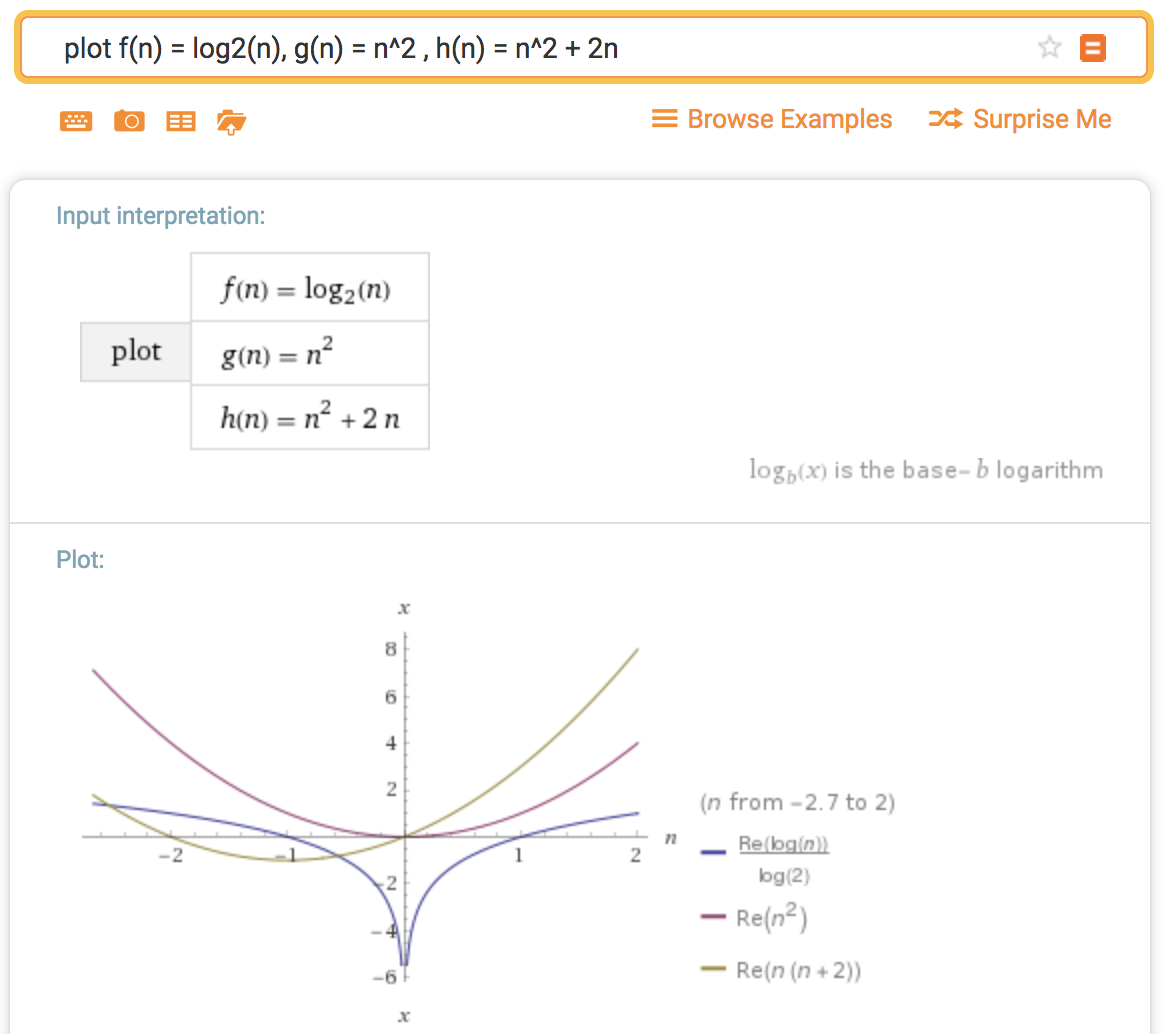
\includegraphics[width=8cm]{del1a.png}
\end{figure} \\ \\
Til sidst kan S3 benyttes til afgøre
størrelsesordenen mellem $f(n) = log_2(n)$ og $g(n) = n^2$. \\ \\ \\
Størrelsesordenen mellem $g(n)$ og $f(n)$ er:
\[ f(n) < g(n) \]
%
%
\newpage
\subsection{DEL 1B}
\[ f(n) = n \sqrt{n} \ og \ g(n) = nlog_{2}(n) + 100n \] \\
%
f(n) kan skrives som 
\[ f(n) = n^{\frac{3}{2}} \]
g(n) skal forkortes, så vi ser på størrelsesordenen mellem
\[ nlog_{2}(n) \ og \ 100n \]
Vi ved efter S2, at en konstant $100$ er af lavere størrelsesorden end 
$log_{2}(n)$ for alle a > 0.
Og fra S8 ved vi, at $n100$ er af lavere end $nlog_{2}(n)$.
Derfor kan vi opskrive g(n) på følgende måde: $g(n) = log_{2}(n)$. \\
Efter S3 kan vi til sidst finde, at g(n) er af lavere størrelsesorden end f(n). \\ \\
Størrelsesordenen mellem $f(n)$ og $g(n)$ er \\
\[ f(n) > g(n) \]

\bigskip
\subsection{DEL 1C}
\[ f(n) = 2^{\log_3(n)} \ og \ g(n) = \frac{2^n}{n^{100}} \] \\
%
Vi ved fra S6, at 
\begin{quotation}
"$x^a$ er af lavere størrelsesorden end $b^x$ (a > 1, b > 1)" \\
\end{quotation}
Da $2^n$ er af lavere størrelsesorden end $n^{100}$ kan vi vide, at
g(n) går mod 0. Vi kan også se, at f(n) går mod uendelig. Vi kan skrive følgende:  
\[ \lim_{n \to \infty} 2^{\log_3(n)} = \infty \]
\[ \lim_{n \to \infty} \frac{2^n}{n^{100}} = 0 \] \\
Størrelsesordenen mellem $f(n)$ og $g(n)$ er \\
% \[ f(n) > g(n) \]
\bigskip
\subsection{DEL 1D}

\[ f(n) = (n + log_2(n))^2 \ og \ g(n) = n^2 \] \\
% 

Vi kan dividere med kvadratroden i begge funktioner, da det ikke
vil ændre størrelsesforholdet mellem de to funktioner.
\[ f(n) = \sqrt{(n + \log_2(n))^2} \ og \ g(n) = \sqrt{n^2} \]
Vi har så, at 
\[ f(n) = n + \log_2(n) \ og \ g(n) = n^2 \]
Herefter skal $f(n)$ forkortes, sådan at vi finder ud af hvilken
størrelsesorden $n$ har i forhold til $\log_2(n)$. 
Efter S3 er $\log_2(n)$ af lavere størrelsesorden end $n^1$, hvorfor vi kan 
skrive $f(n)$ og $g(n)$ således:
\[ f(n) = n \ og \ g(n) = n^2 \] \\
Efter S5 er $n^1$ af lavere størrelsesorden end $n^2$, hvorfor vi har, at: \\ \\
%
Størrelsesordenen mellem $f(n)$ og $g(n)$ er 
\[ f(n) < g(n) \] \\ \\
%






\newpage
\section{DEL 2}

%
%%%% OPGAVETEKST 
%
{\bfseries Vi betragter fire følger givet ved henholdsvis}
\newline $a_{1}$ = 2, $a_{2}$ = 200, $a_{n}$ = $a_{n-2}$ for n \geq 3
\newline $b_{1}$ = 2, $b_{n}$ = $b_{n-1}+2$ for n \geq 2
\newline $c_{1}$ = 1, $c_{n}$ = $nc_{n-1}$ for n \geq 2
\newline $d_{n}$ = $log_{2}(c_{n})$ hvor $c_{n}$ er defineret som oven over og n \geq 1. 

\subsection{DEL 2A}
For hver af de 3 rekursive følger $a_{n}$, $b_{n}$ og $c_{n}$, find et eksplicit udtryk for det n't led. Det vil sige, find funktioner $f_{a}(n)$, $f_{b}(n)$, $f_{c}(n)$ således $a_{n} = f_{a}(n)$, 
$b_{n} = f_{b}(n)$, $c_{n} = f_{c}(n)$.

\bigskip 
\noindent
$a_{n}$ = $a_{n-2}$ for n \geq 3
\newline $a_{1}$ = 2
\newline $a_{2}$ = 200
\newline $a_{3}$ = $a_{3-2}$ = $a_{1} = 2$
\newline $a_{4}$ = $a_{4-2}$ = $a_{2} = 200$
\newline $a_{5}$ = $a_{5-2}$ = $a_{2} = 2$
\newline $a_{6}$ = $a_{6-2}$ = $a_{4} = 200$

\noindent
\newline\newline
Af ovenstående ses et mønster, hvor der i tilfælde af det n'te led i følgen er et ulige tal, er det korresponderende  indekstal 2. Omvendt, hvis det n'te led i følgen er et lige tal er indekstallet 200. 

\noindent
\newline\newline
Ud fra dette mønster kan vi danne følgende funktion: 

\noindent
\bigskip
$f_{a}(n)$ = $\left\{\begin{array}{cc} 2 \mbox{~hvis~} n-2\lfloor{\frac{n}{2}}\rfloor = 1 \\
200 \mbox{~hvis~} n-2\lfloor{\frac{n}{2}}\rfloor = 0 \end{array}\right.$

\bigskip
\noindent
$b_{n}$ = $b_{n-1} + 2$ for n \geq 2
\newline $b_{1}$ = 2
\newline $b_{2}$ = $b_{2-1} + 2$ = $b_{1} + 2$ = 2 + 2 = 4
\newline $b_{3}$ = $b_{3-1} + 2$ = $b_{2} + 2$ = 4 + 2 = 6
\newline $b_{4}$ = $b_{4-1} + 2$ = $b_{3} + 2$ = 6 + 2 = 8

\noindent
\newline
Ud fra dette mønster kan vi danne følgende funktion: $f_{b}(n) = 2n$

\bigskip
\noindent
$c_{n}$ = $nc_{n-1}$ for n \geq 2
\newline $c_{1}$ = 1
\newline $c_{2}$ = $2c_{2-1}$ = $2c_{1}$ = 2 * 1 = 2
\newline $c_{3}$ = $3c_{3-1}$ = $3c_{2}$ = 3 * 2 = 6
\newline $c_{4}$ = $4c_{4-1}$ = $4c_{3}$ = 4 * 6 = 24
\newline $c_{5}$ = $5c_{5-1}$ = $5c_{4}$ = 5 * 24 = 120

\noindent
\newline
Ovenstående følge er også kendt som fakultetsfølgen. Derfor bliver $f_{c}(n) = n!$

\subsection{DEL 2B}
Husk på, at vi siger ($a_{n}$) er $\Theta(b_{n})$, hvis følgen ($a_{n}$) er af samme størrelsesorden som følgen ($b_{n}$). For hver af de 3 følger ($a_{n}$), ($b_{n}$) og ($d_{n}$), find en tilsvarende størrelsesorden fra nedensåtende liste der korrekt beskriver følgens størrelsesorden: 
\newline $\Theta(1), \Theta(n), \Theta(nlog_{2}(n)), \Theta(n^{2}), \Theta(2^{n})$
\newline
Argumentér for konklusionerne ud fra notesættets sætninger og regler (O1-O9, S1-S9). 

\bigskip
\noindent
$f_{a}(n)$ = $\left\{\begin{array}{cc} 2 \mbox{~hvis~} n-2\lfloor{\frac{n}{2}}\rfloor = 1 \\
200 \mbox{~hvis~} n-2\lfloor{\frac{n}{2}}\rfloor = 0 \end{array}\right.$

\bigskip
\noindent
Ovenstående funktion er en relativt simpel funktion, hvor outputtet kun kan være 2 eller 200. Dermed giver et input, hvor n $\geq$ 1 et øjeblikkeligt output uden yderligere bearbejdning, hvorfor der kun er 1 trin for denne funktion. Af den årsag er $\Theta(1)$ af samme størrelsesorden som $f_{a}(n)$. %%%%%%%%%%%%%%% Er det svar nok? Og er det overhovedet et korrekt svar? Hvilken O1-O9/S1-S9 passer denne overens med? :| 

\bigskip
\noindent
Sætning S7 foreskriver, at cf(x) er af samme størrelsesorden som f(x) når c $\neq$ 0. Funktionen $f_{b}(n) = 2n$, hvor c = 2 og derfor ikke 0. Dermed er $\Theta(n)$ af samme størrelsesorden som $f_{b}(n)$

\bigskip
\noindent
$d_{n} = log_{2}(c_{n}) = log_{2}(n!)$ hvor $c_{n}$ er defineret som oven over og n $\geq$ 1. \\
Sætning 17 foreskriver, at $log_{2}n!$ er $\Theta(nlog_{2}(n))$. Dermed er $\Theta(nlog_{2}(n))$ af samme størelsesorden som $log_{2}(c_{n})$. 



\section{DEL 3}
Find udtryk for køretid (antal af udførte instruktioner) af COMPUTE(n) ved input n $\geq$ 1 som en rekursiv følge $(t_{n})$. Du kan antage at hver linje af programmet svarer til en instruktion når du tæller instruktioner. Hvilken af $\Theta$-notationerne fra Eq. (1) beskriver køretid af COMPUTE(n)?

\bigskip
\hfill Times
\newline
\noindent
function Compute(n) \hfill n
\newline
\indent 
if n = 1 then \hfill n
\newline
\indent\indent
return n \hfill 1
\newline
\indent
else \hfill n-1
\newline
\indent\indent
return n*Compute(n-1) \hfill n-1

\bigskip
\noindent
T(n) = n + n + 1 + (n - 1) + (n - 1) = 2(n) + 2(n-1) + 1 = O(n)

\end{document}